\documentclass[conference,compsoc]{IEEEtran}

\usepackage{graphicx}
\usepackage{subcaption}
\usepackage{calc}
\def\scalecaption{\normalsize}

\setcounter{figure}{4}

\begin{document}

\begin{figure}[ht]
    \begin{subfigure}[b]{0.48\columnwidth}
        \centering
        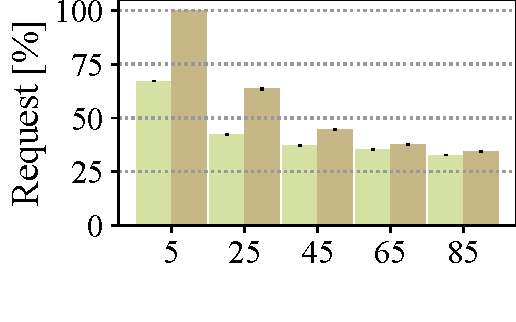
\includegraphics[trim={0 22pt 0 0}, clip, width=1.0\linewidth]{sp_sub/sub_line/subsampling_equal-ncd_dpk-gurobi_04_gm:GM_scatter_legend}
        %
        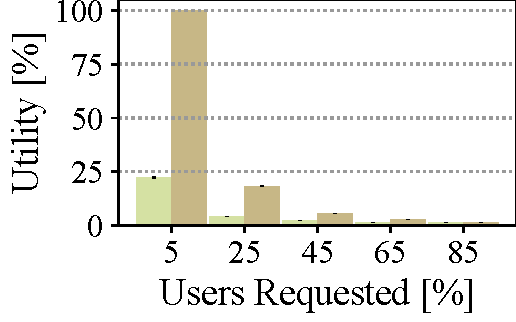
\includegraphics[width=1.0\linewidth]{sp_sub/sub_line/subsampling_ncd_dpk-gurobi_04_gm:GM_scatter_legend}
        \caption{W1:GM}

    \end{subfigure}
%
    \begin{subfigure}[b]{0.48\columnwidth}
        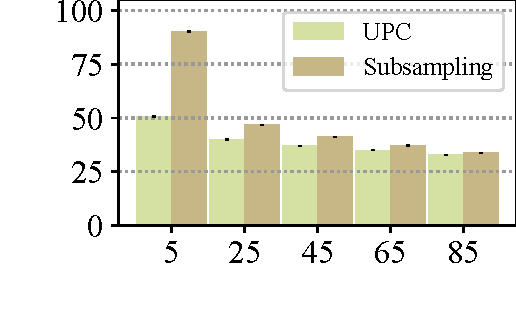
\includegraphics[trim={20pt 22pt 0 0}, clip, width=\dimexpr\linewidth-9pt\relax]{sp_sub/sub_line/subsampling_equal-ncd_dpk-gurobi_04_basic:GM-LM-RR-LSVT_scatter_legend}
        %
        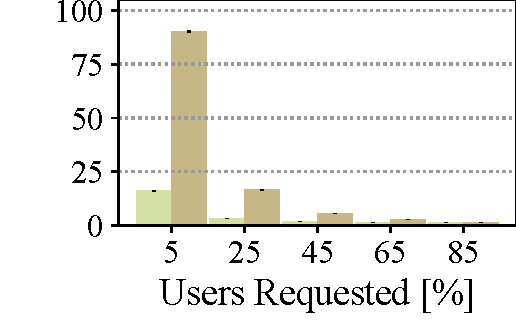
\includegraphics[trim={20pt 0 0 0}, clip, width=\dimexpr\linewidth-9pt\relax]{sp_sub/sub_line/subsampling_ncd_dpk-gurobi_04_basic:GM-LM-RR-LSVT_scatter_legend}
        \caption{W2:Mix}
    \end{subfigure}
%
    \caption{Comparing UPC with Poisson subsampling on two workloads, varying the fraction of the selected population.}
    \label{fig:sub}
\end{figure}


\end{document}
